\chapter{Développement d'outils d'investigation}
\label{chap:2}
\section{Méthode de modélisation au niveau système}

% Need to simulate from source to input for soft-failure analysis
Une méthodologie de construction de modèles ESD au niveau système est proposée.
Elle permet une simulation précise jusqu'à l'entrée d'un circuit intégré en fonctionnement.
Un environement de test ESD est composé d'éléments récurrents tels que des sources DC, des oscilloscopes, et des générators stress, interconnectés par des cables et des fils.
Les cartes électroniques embarquent différents types de composants, tels que des passifs, des protections ESD, des chokes.
L'objectif de la méthode proposée est de construire une librairie des éléments les plus courants, puis d'assembler le modèle complet du système avec.

% Cables and delays identified as important for esd sims - because of similar order of magnitude
Les cables sont des éléments importants mais parfois négligés dans les simulations ESD.
Ils introduisent des délais de propagation non négligeables par rapport à la durée d'un ESD.
Pour ordre de grandeur, un cable coaxial 50\textOmega{} possède une constante de propagation d'environ 5 ns/m.
En comparaison, un ESD dure entre une dizaine et plusieurs centaines de nanosecondes, ce qui est globablement proche du même ordre de grandeur.
Les câbles sont avant tout des lignes de transmission, dont l'analyse théorique fut faite par J. Maxwell, L. Kelvin et O. Heavyside et énormément étudiées par la suite dans la littérature \cite{branin-tl-ref, hf-coax,lossy-tl,emc-analysis-tl}.

% Distributed model
Dans le domaine de ESD, le modèle le plus populaire de ligne est basé sur des éléments distribués.
Concrètement, c'est une suite réseaux L-C tels que la Fig. \ref{fig:dis-line-model}.
Les valeurs de chaque élément sont calculées à partir des propriétés du cable et de la précision requise pour la simulation.

\begin{figure}[!h]
  \centering
  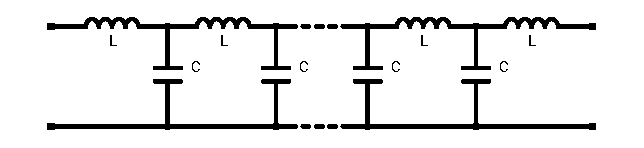
\includegraphics[width=0.7\textwidth]{src/2/figures/lc_ladder.pdf}
  \caption{Electrical distributed LC ladder model of a lossless transmission line}
  \label{fig:dis-line-model}
\end{figure}

% Perks and disavantages
Malgré sa très large adoption, ce modèle présente de sérieux inconvénients.
En particulier, ce modèle nécessite un très grand nombre d'éléments pour avoir une précision décente.
Pour une même précision, le nombre d'éléments est proportionnel à la longueur du cable, ce qui augmente considérablement les temps de simulation.
Pour augmenter la bande passante du modèle, le nombre d'éléments doit également être augmenté.
La combinaison des deux résulte en des temps de simulation très longs.

% Behavioral model
Le modèle à deux ports décrit par H. Branin \cite{branin-tl-ref} est une alternative bien plus sérieuse au modèle distribué.
Il décrit très efficacement et avec une très grande précision le comportement d'une ligne de transmission.
La bande passante n'est pas limité, et le temps de simulation est indépendant de la longueur du câble.
Le modèle est constitué de deux sources de tension controllées en tension et deux résistances (Fig. \ref{fig:beh-line-model}).

\begin{figure}[!h]
  \centering
  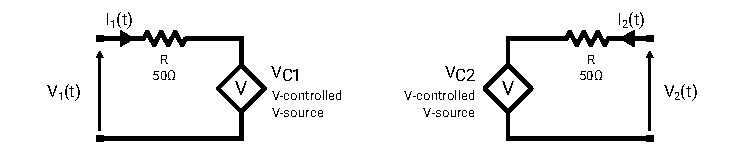
\includegraphics[width=\textwidth]{src/2/figures/behavioral_line_model.pdf}
  \caption{Electrical behavioral model of a lossless transmission line}
  \label{fig:beh-line-model}
\end{figure}

Le comportement des sources est décrit par les équations \ref{eq:beh-line-1} et \ref{eq:beh-line-2}.

\begin{equation}
V_{C1}(t) = V_{2}(t - \Delta t) + Z_{C}.I_{2}(t - \Delta t)
\label{eq:beh-line-1}
\end{equation}

\begin{equation}
V_{C2}(t) = V_{1}(t - \Delta t) + Z_{C}.I_{1}(t - \Delta t)
\label{eq:beh-line-2}
\end{equation}

% Explain the equations
Z\textsubscript{C} est l'impédance charactéristique de la ligne et \textDelta{}t le délai de propagation.
Les équations décrivent un système où tension et courant à chaque port sont la superposition d'une onde se propageant dans un sens et d'une seconde dans l'autre sens.

% Compare both models to know which one is preferrable
Des simulations permettent de comparer les deux modèles.
Une impulsion rectangulaire est injectée sur chaque modèle avec un temps de montée de 1ps.
Différentes charges permettent d'évaluer les performances et la précision.
Les lignes de transmission ont un délai de 100ns et une impédance charactéristique de 50\textOmega{}.

\begin{figure}[!h]
  \centering
  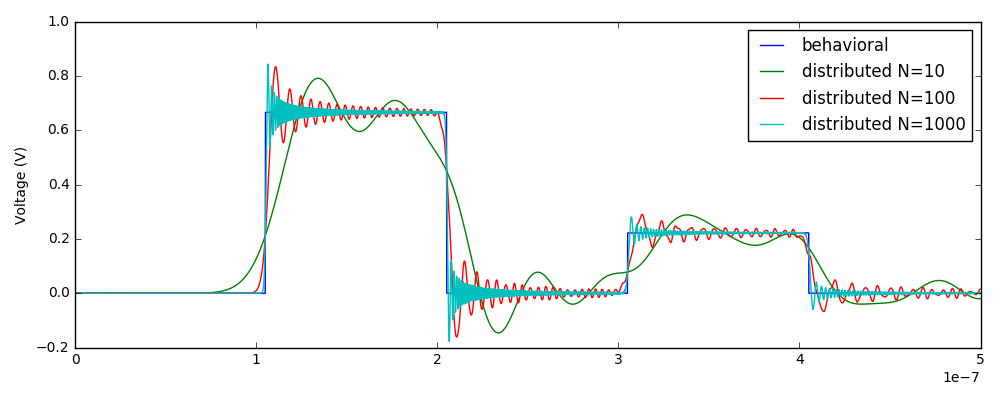
\includegraphics[width=0.3\textwidth]{src/2/figures/tline_comparison.pdf}
  \caption{Lumped versus two-port models comparison in simulation}
  \label{fig:lines-simulations}
\end{figure}

Le modèle comportemental surpasse le modèle distribué, autant en précision que temps de simulation.
Il reproduit parfaitement le temps de montée avec toutes les charges (Fig. \ref{fig:lines-simulations}).
Il est plus rapide à simuler de plusieurs ordres de grandeurs par rapport au modèle distribué.

La modélisation d'autres éléments importants tels que les composants passifs et les protections ESD est détaillé dans le document complet.

% Illustrate the method with a practical case
Pour illustrer l'application de la méthode de modélisation, elle est appliquée sur un banc TLP du laboratoire de NXP Toulouse.
C'est un bon cas d'étude afin d'utiliser la méthode, car ce banc est très largement utilisé pour l'investigation.
Pour démontrer sa précision, le modèle est vérifié par comparaison avec de multiples mesures, sous différentes charges et amplitudes.

\begin{figure}[!h]
  \centering
  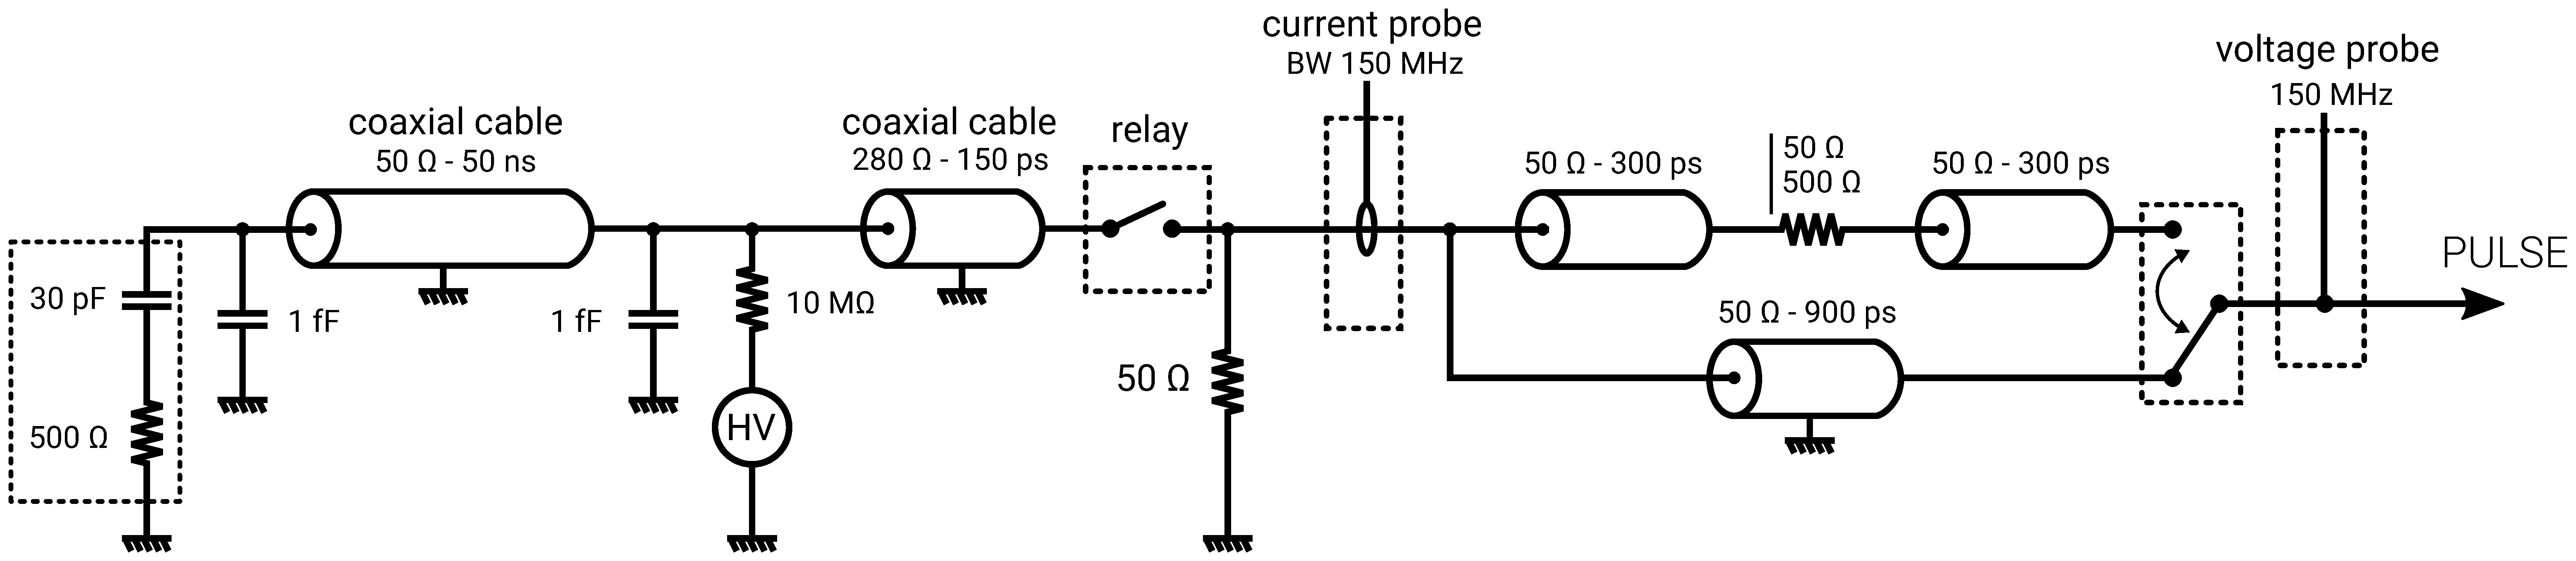
\includegraphics[width=\textwidth]{src/2/figures/complete_nxp_tlp_model.pdf}
  \caption{Complete model of NXP laboratory's TLP generator}
  \label{fig:complete-tlp-model}
\end{figure}

% Explain how the model, how it was constructed
Le modèle complet de TLP est donné en Fig. \ref{fig:complete-tlp-model}.
Il reproduit l'architecture du TLP du laboratoire en utilisant des modèles de la librairie pour chaque élément.
% Detail a first comparison with 25 ohms
Une première validation avec une mesure est donnée en Fig. \ref{fig:comparison-tlp-load}.
Avec une charge de 25\textOmega{} et une tension de charge de 500V, 4.5A et 125mV sont relevés sur le second plateau.
Le rapport de ces deux valeurs corresponds bien à 25\textOmega{} comme attendu.
Jusqu'à 220 ns, les deux courbes se ressemblent fortement.
Après, des différences apparaissent à cause des ondes réfléchies, qui entrainent une accumulation d'erreurs.
La plupart des simulations ESD restent intéressantes pendant la partie principale de la décharge jusqu'à 120ns et ces erreurs sont donc négligeables.

\begin{figure}[!h]
  \centering
  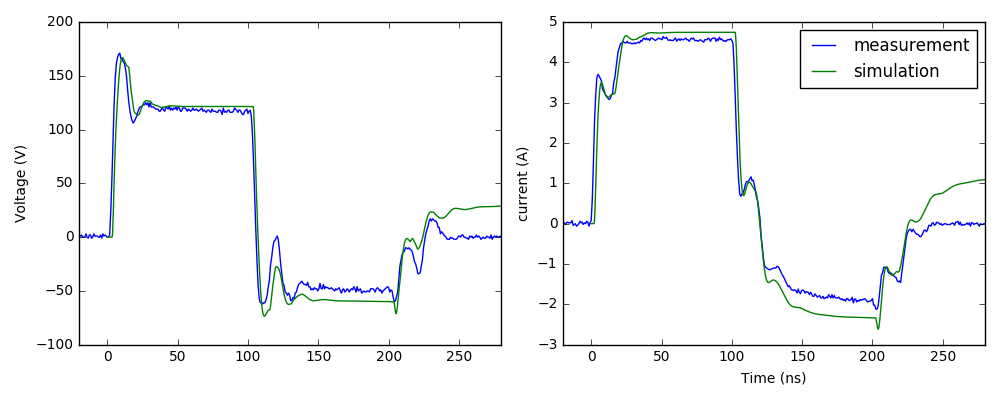
\includegraphics[width=\textwidth]{src/2/figures/tlp_comparison_R25_500V.png}
  \caption{Voltage and current waveforms comparison - 500 V charging voltage on 25\textOmega{}}
  \label{fig:comparison-tlp-load}
\end{figure}

% More validations in Annex
Les autres validations sont données dans le document complet, et présentent des niveaux de corrélations aussi proches.
Le modèle fonctionne correctement et reproduit les mesures, prouvant sa validité.

\section{Dévelopement d'un générateur TLP modifié}

%TODO: Simplifier
% TLP is a great tool for esd analysis
A travers cette étude et de manière générale, le TLP est utilisé très largement comme outil de characterization et de test.
Il est capable de générer des impulsions très bien controllées et reproductibles.
Néanmoins, il ne reproduit pas les formes d'ondes ESD rencontrés dans la réalité.
C'est pourquoi l'utilisation des pistolets ESD reste obligatoire pour la qualification de produits.
La forme d'onde la plus répandue est celle définie dans la spécification HMM \cite{hmm} et les standards IEC 61000-4-2 \cite{iec61000-4-2} et ISO 10605 standard \cite{iso10605}.
Ensemble, ils couvrent une très large plage d'applications, dans les domaines grand-public, automobile et industriel.
Pour combiner les avantages d'un TLP avec ceux d'une décharge HMM, un générateur TLP peut être modifié pour produire cette impulsion HMM.
Cette approche a été explorée par le passé par E. Grund \cite{iec61000-tlp} et Y. Cao \cite{tlp-based-hmm}.
Néanmoins, leurs techniques présentent quelques inconvénients tels que une tendance large à créer des oscillations, comme démontré dans le document complet.

Le générateur proposé ici est dénommé TLP-HMM.
Le TLP-HMM requiert deux modules additionnels à connecter à chaque extrémité d'un TLP standard 100ns.
Ils sont nommés \textit{absorber} et \textit{shaping filter} (Fig. \ref{fig:tlp_hmm_architecture}).
Le principe du TLP-HMM est de rerouter une portion du courant incident dans la masse, de manière à ce que le courant restant prenne la forme de l'onde HMM.

\begin{figure}[!h]
  \centering
  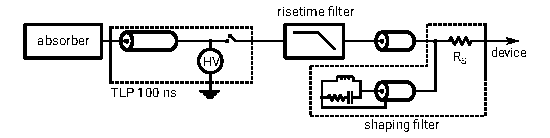
\includegraphics[width=0.9\textwidth]{src/5/figures/beges_tlp_hmm.pdf}
  \caption{TLP-HMM architecture}
  \label{fig:tlp_hmm_architecture}
\end{figure}

% Role of the shaping filter
Le shaping filter (Fig. \ref{fig:shaping_filter_example}) dévie le courant nécessaire pour former l'onde.
Il est composé de cinq éléments, un réseau RLC, un petit câble coaxial de délai \textDelta{}t, et une résistance d'injection.

\begin{figure}[!h]
  \centering
  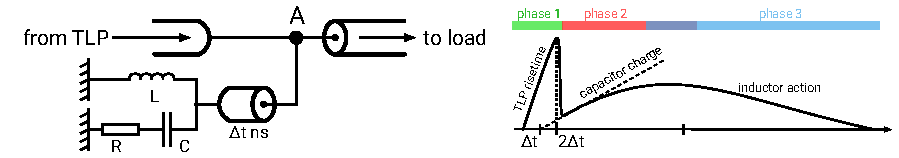
\includegraphics[width=0.98\textwidth]{src/5/figures/example_tlp_hmm.pdf}
  \caption{Shaping filter architecture and operation}
  \label{fig:shaping_filter_example}
\end{figure}

% Behavior of the filter - C
Une impulsion TLP rectangulaire est injectée sur la ligne principale (Fig. \ref{fig:shaping_filter_example}).
Elle atteint le point A à $t=0$ et la tension monte.
La capacité ne voit l'impulsion a $t=\Delta t$, et ne se charge que à partir de ce moment.
En retour, la charge est visible sur la ligne principale seulement à $t=2\Delta t$.
A cet instant, le potentiel chute sur la ligne principale, car la capacité devient visible et tire tout le courant.
Le premier pic de l'impulsion est ainsi créé, avec une durée d'environ $2\Delta t$.

% Behavior of L
Pendant que la capacité continue de se charger, l'inductance connectée en parallèle commence à absorber du courant à son tour.
A un moment donné, elle absorbe suffisamment de courant pour contrecarrer la charge de la capacité, et la tension commence à redescendre.
La décharge se poursuit lentement jusqu'à retourner à une tension nulle.
Le résultat de toutes ces actions est la création de la forme d'onde complète du HMM.

% Introduce the design
Le schéma exact du shaping filter est donné Fig. \ref{fig:shaping_filter_schematic}.
Le capacitance totale est distribuée pour réduire l'inductance parasite.
Les inductances sont également distribuées pour augmenter la capacité en courant.

\begin{figure}[!h]
  \centering
  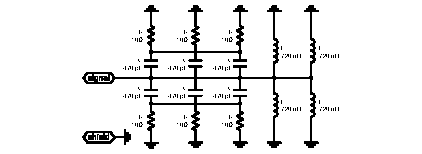
\includegraphics[width=0.9\textwidth]{src/5/figures/shaping_filter_schematic.pdf}
  \caption{shaping-filter schematic}
  \label{fig:shaping_filter_schematic}
\end{figure}

A la fin de la décharge, l'inductance continue d'absorber un courant important.
Si rien n'est fait, le potentiel au point pourrait être tiré négativement.
Pour empêcher cela, l'absorbeur lisse le front descendant de l'impulsion TLP sur une centaine de nanosecondes.
En ramenant doucement le courant à zéro, l'inductance s'arrête lentement d'absorber du courant et la tension reste nulle sans devenir négative.
La schématique de l'absorbeur est donnée Fig. \ref{fig:absorber_schematic}

\begin{figure}[!h]
  \centering
  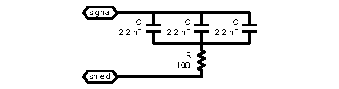
\includegraphics[width=0.7\textwidth]{src/5/figures/absorber_schematic.pdf}
  \caption{absorber schematic}
  \label{fig:absorber_schematic}
\end{figure}

Les courbes simulées et mesurées sur un prototype sont données Fig. \ref{fig:tlp_hmm_waveforms}.
Les courants mesurés à 30ns et 60ns sont dans la marge de tolérance de 30\% des standards, et elle est donc valide.

\begin{figure}[!h]
  \centering
  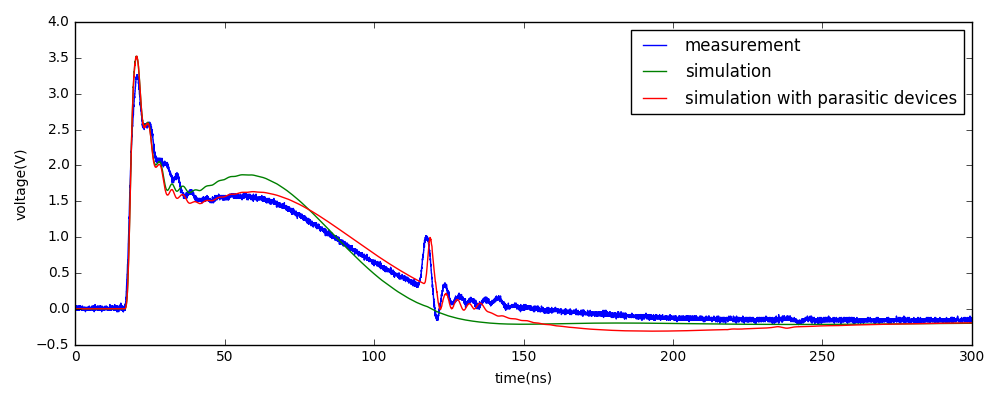
\includegraphics[width=0.95\textwidth]{src/5/figures/tlp_hmm_waveforms.png}
  \caption{Measurement versus simulation of a 250V TLP-HMM (equivalent 1kV HMM) on 2\textOmega{}}
  \label{fig:tlp_hmm_waveforms}
\end{figure}

% Analyse the curve
Globalement, la simulation et la measure corrèlent bien.
Il y a des différences mineures, notamment entre 40ns and 150ns.
Elles sont dues à des éléments parasites non pris en compte durant les simulations, et des corrections sont à apporter au prototype.
L'analyse de ces éléments est fournie dans le document complet.

% Conclusion regarding TLP-HMM
Une nouvelle méthode pour générer des impulsions HMM avec un générateur TLP a été présentée.
Ce TLP-HMM fonctionne correctement, passe les conditions des standards avec succès et s'avère robuste contre les oscillations et perturbations externes.
Le prototype permet de valider le concept.
Le design doit être amélioré pour éliminer des éléments parasites.
Une tension de charge plus élévée doit aussi être disponible pour augmenter la capacité en courant du générateur actuellement limitée à 4A.

\section{Méthode de traitement de capteurs de courant on-chip}

% Introduction
Near-field scan has been presented previously in \ref{sec:near-field-scan}.
Using this technique it is possible to measure maps of electric or magnetic field above a device.
While those maps already provide interesting information, to locate sources of RF noise for instance, it is interesting to post-process them in order to get voltages and currents inside the measured circuit.
In this section, two different methods are described for reconstructing the original current from a near-field magnetic measurement.
Each method requires a preliminary characterization of the probe.
Near-field scanners were extensively studied in \cite{near-field-scan, phd-monnereau}.

% What is the output voltage that is measured
It is shown in \cite{near-field-scan} that the measured voltage of near-field magnetic probe is proportional to the time derivative of the measured and coupled current.
In the next part of this analyis, the sensor voltage is denoted V\textsubscript{sensor} and the original current I\textsubscript{TLP}.

it is possible to express I\textsubscript{TLP} as a function of the measured sensor voltage V\textsubscript{sensor}.
This is expressed in Eq. \ref{eq:nfs-rel2}.
The offset $A$ is the result of the integration.

\begin{equation}
I_{TLP}(t) = \frac{1}{G}\int V_{sensor}(t) \mathrm{d}t + A
\label{eq:nfs-rel2}
\end{equation}

% How to determine 1/G and A
Both constants $1/G$ and $A$ are determined experimentally with a preliminary calibration.
Once calculated, both factors are estimated to remain constant and can be reused in other measurements.

% Talk about calibration setup
On silicon, one of the sensors is dedicated to the calibration phase.
The setup is given in Fig. \ref{fig:calibration-sensor}.
The input of the sensor is represented by ports S1 and S2.
A square impulse of 1V amplitude generated by a 100ns wide TLP with a risetime of 8ns is injected between the two input pins.
The response V\textsubscript{sensor} is measured with a 2GHz bandwith 10GS/s oscilloscope in differential input connected between C1 and C2.

\begin{figure}[!h]
  \centering
  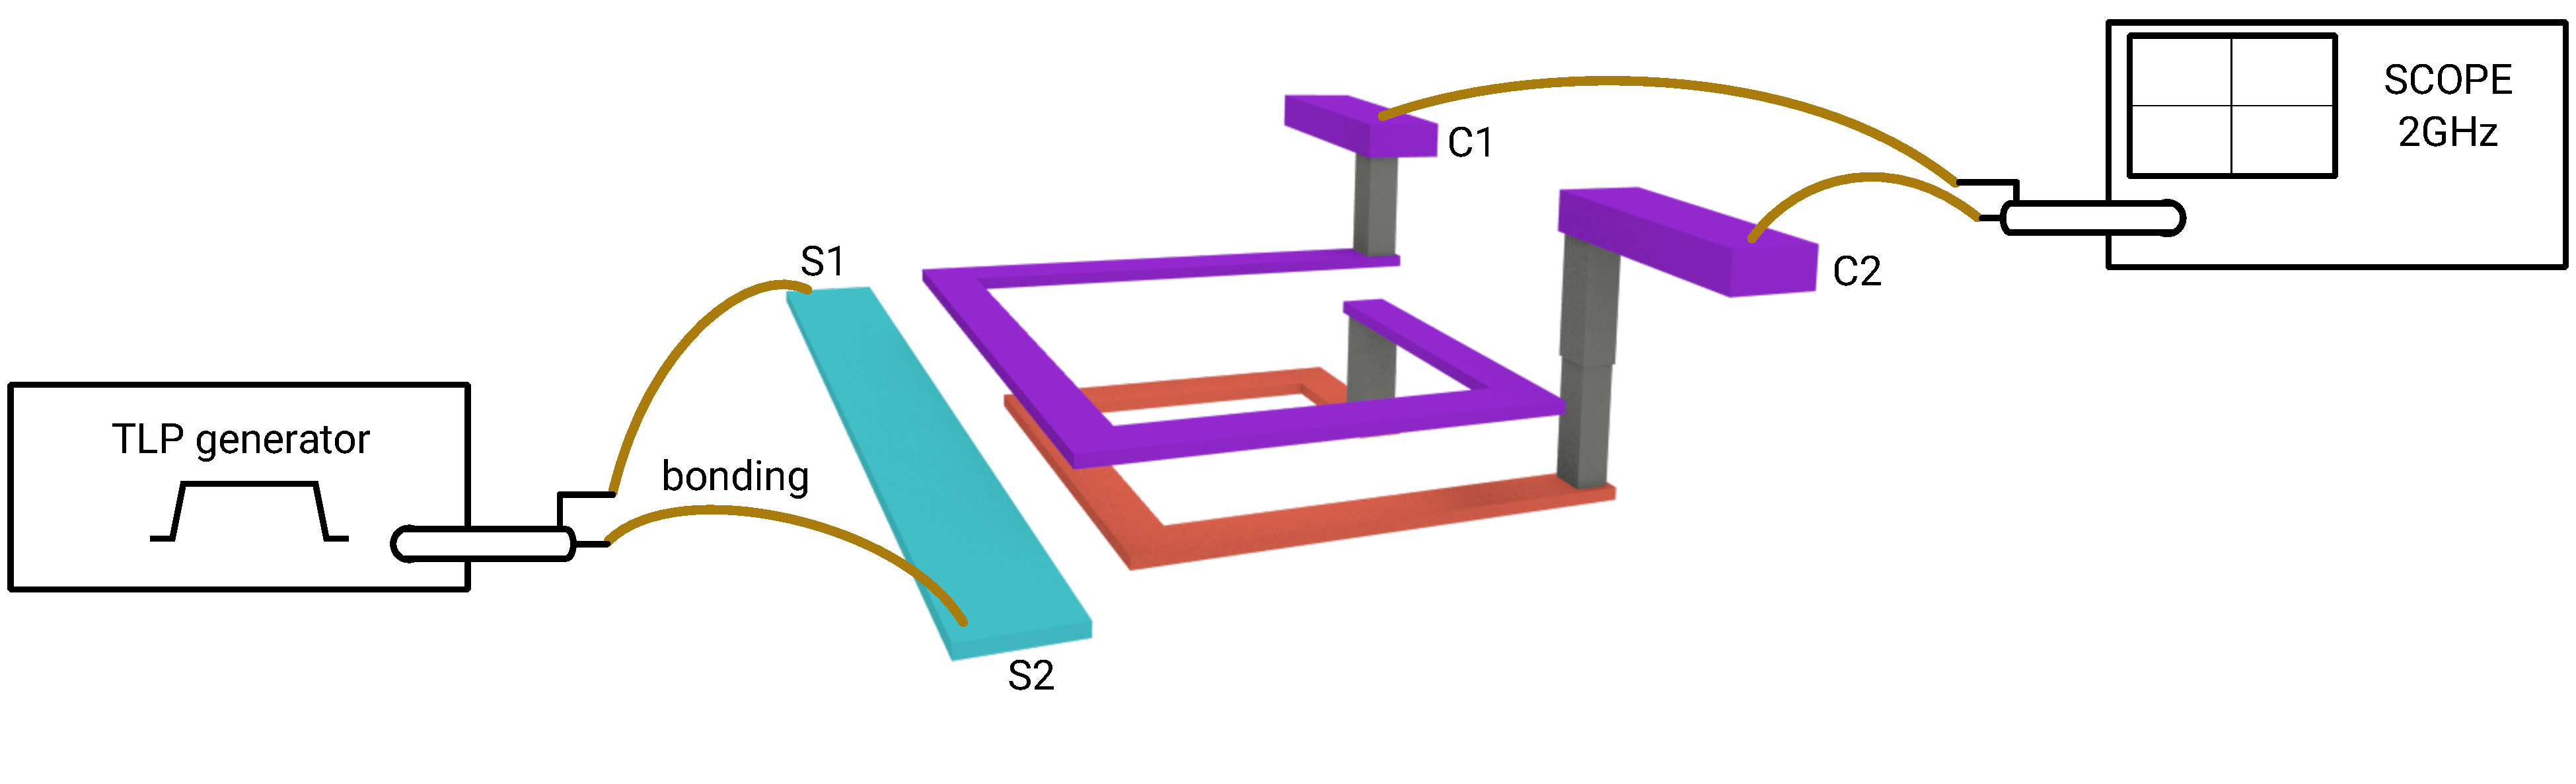
\includegraphics[width=0.9\textwidth]{src/3/figures/sensor_measurement_setup.pdf}
  \caption{Calibration sensor setup for time-domain method}
  \label{fig:calibration-sensor}
\end{figure}

% Explain the measurements
I\textsubscript{TLP} and V\textsubscript{sensor} waveforms are recorded during calibration (see Fig. \ref{fig:measurement-nfs}).
The top curve represents the input (I\textsubscript{TLP}) and the bottom curve the output (V\textsubscript{sensor}).

\begin{figure}[!h]
  \centering
  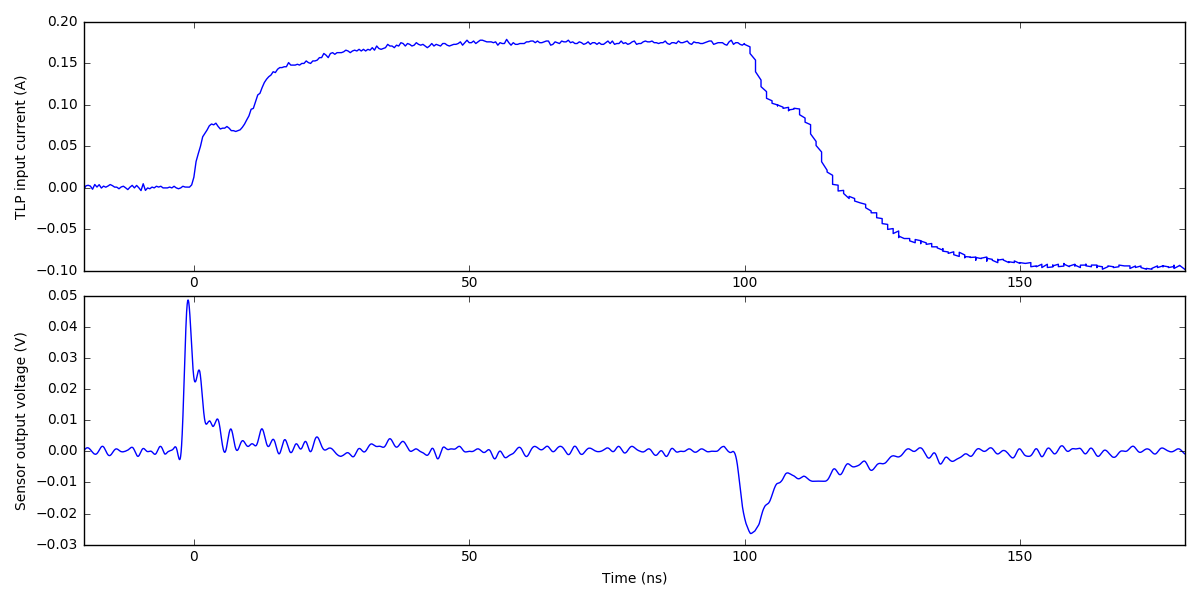
\includegraphics[width=0.95\textwidth]{src/3/figures/measured_waveform.png}
  \caption{Measured voltage waveform}
  \label{fig:measurement-nfs}
\end{figure}

% Integration method
With those measurements, $1/G$ and $A$ are determined experimentally.
Both values were estimated at $1/G = 8.10^8$ and $A = -V_{TLP}(t = 0)$.

% Intro & Characterization
The frequency-domain method post-processes the V\textsubscript{sensor} waveform using the sensor's frequency response.
The characterization is conducted with the calibration sensor, using a \gls{vna}.
The calibration setup is similar to the time-domain method.
It is given in Fig. \ref{fig:calibration-sensor-rf}.

\begin{figure}[!h]
  \centering
  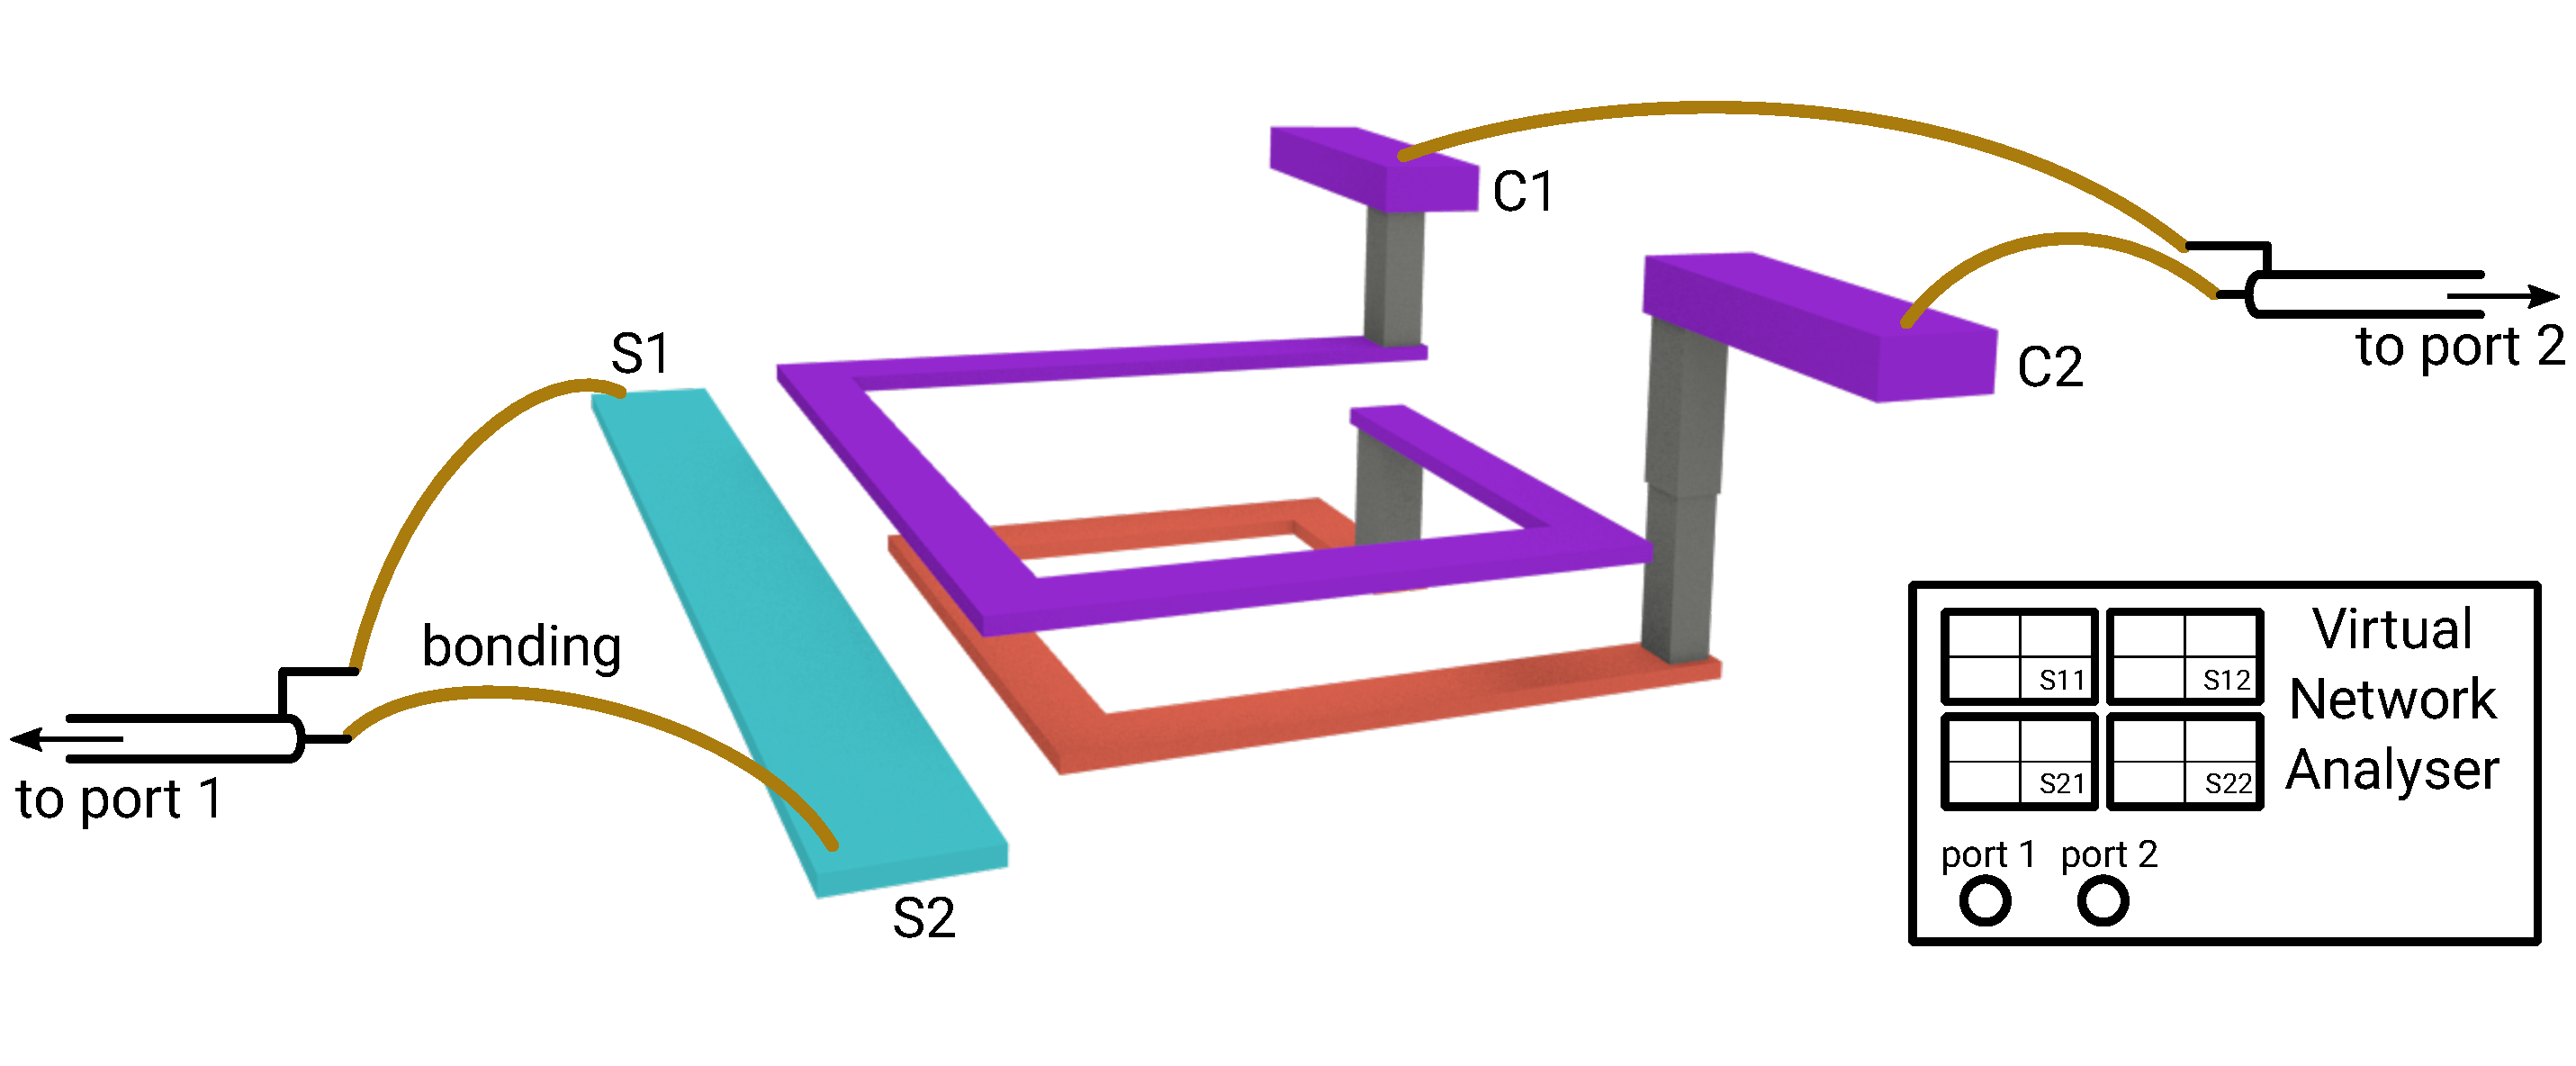
\includegraphics[width=0.9\textwidth]{src/3/figures/sensor_measurement_setup_rf.pdf}
  \caption{Calibration sensor setup for time-domain method}
  \label{fig:calibration-sensor-rf}
\end{figure}

% Detail characterization
The \gls{sparams} measurements of the sensor are given in Fig. \ref{fig:sensor-response}.
$S11$ is the reflected power at port 1.
$S21$ is the transmitted power between port 1 and port 2, and $S12$ is the transmitted power between port 2 to 1.
In theory, $S12$ is identical to $S21$ for symetrical 2-port devices.
$S22$ is the reflected power from the output, which is not relevant for this study.

\begin{figure}[!h]
  \centering
  \includegraphics[width=0.9\textwidth]{src/3/figures/sensor_freq_response.png}
  \caption{Sensor frequency response}
  \label{fig:sensor-response}
\end{figure}

% Analyse the response
It was suspected previously that the sensor's response is not constant versus frequency.
The \gls{sparams} measurement confirms it, showing a sensor bandwidth of about 300MHz.

% Talk about S11
S11 shows a resonance of -43.9 dB at 1.15 GHz.
It corresponds to a frequency where insertion losses become very small.
However, this peak is not visible on the transmitted coefficient $S12$ or $S21$.
It probably means that at this frequency, a part of the input power is dissipated by the device, either by the bonding or the sensor itself.


\begin{figure}[!h]
  \centering
  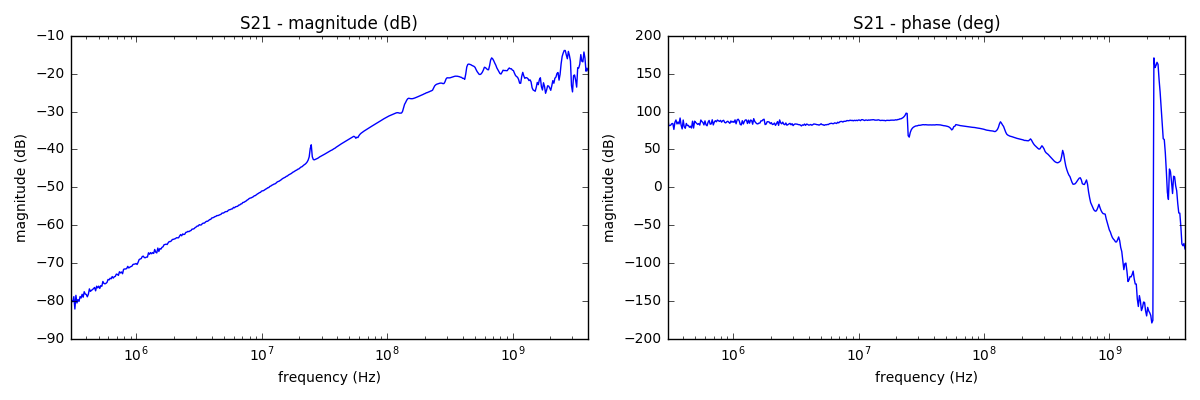
\includegraphics[width=0.9\textwidth]{src/3/figures/s21_freq_response.png}
  \caption{Sensor frequency response - complex S21 (magnitude and phase)}
  \label{fig:s21-response-complex}
\end{figure}

\begin{figure}[!h]
  \centering
  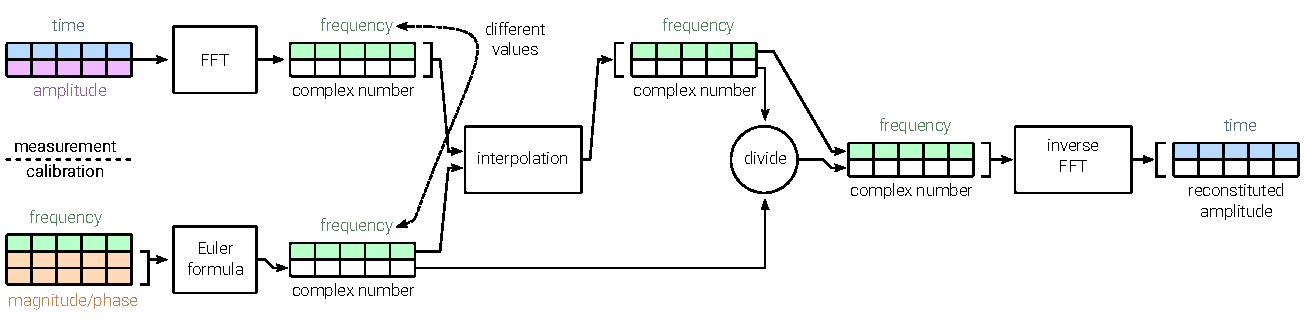
\includegraphics[width=\textwidth]{src/3/figures/frequency_post_process_flow.pdf}
  \caption{Post-processing pipeline}
  \label{fig:postprocess-nfs-pipeline}
\end{figure}

% The algorithm
The post-processing method is detailled in Fig. \ref{fig:postprocess-nfs-pipeline}.
The measurement data in the time-domain is converted to the frequency domain using \gls{fft}.
The ouptut array associates to each frequency point a complex number.
An example is given in Table \ref{tab:complex-fft}.

\begin{table}[!h]
  \centering
  \begin{tabular}{@{}lllll@{}}
  \toprule
  frequencies (Hz)        & complex value                \\ \midrule
  1.0*10^6                & 0.33 + i0.2                  \\
  2.0*10^6                & 0.46 - i1.2                  \\
  etc.                    & etc.                         \\ \bottomrule
  \end{tabular}
  \caption{Structure for the result of (complex) FFT}
  \label{tab:complex-fft}
\end{table}

On the other hand, the S21 calibration data associates a phase and magnitude to each frequency point.
An example is given with Table \ref{tab:sparams}.
Using Euleur formula (Eq. \ref{eq:to-complex}), magnitude and phase are converted to a complex number.

\begin{table}[!h]
  \centering
  \begin{tabular}{@{}lllll@{}}
  \toprule
  frequencies (Hz)          & magnitude (dB)         & phase (rad)     \\ \midrule
  1.5*10^6                  & -10                    & 1.23            \\
  2.5*10^6                  & -12                    & 0.12            \\
  etc.                      & etc.                   & etc             \\ \bottomrule
  \end{tabular}
  \caption{Structure for the S-parameter measurement}
  \label{tab:sparams}
\end{table}

\begin{equation} \label{eq:to-complex}
  S21_{complex} = 10^{\frac{magnitude}{20}} * (\cos(phase) + i*\sin(phase))
\end{equation}

% Interpolation step
After these two operations, both data are in the frequency domain.
Before moving forward in the processing, an interpolation step is required.
Indeed, the frequency points between the measurement and the calibration do not match.
For the next part of the algorithm, they need to be identical.
In this case study, a linear interpolation is employed on the measurement data to align it on the characterization.
It is possible that this kind of interpolation is not ideal.
The impact of the interpolation on the results has not been studied yet but it should be done in a future work.

% Compensation
Afterwards, the measurement data is compensated by the characterization data of the sensor.
This is done by dividing each complex value of the measurement by the complex value of the sensor.

% Inverse FFT
Finally, the inverse \gls{fft} of the compensated data is calculated to bring back the waveform into the time-domain.
The resulting waveform is compared to the original and the integration method in Fig. \ref{fig:freq-domain-reconstructed}.
Overall, the results are similar between the time-domain and frequency-domain reconstitutions.
The frequency domain seems to have more dynamic behavior, because it looks like it is reproducing rising and falling edges better.
However, they have both large errors after the pulse and fail to reproduce the reflected wave.
There is a lot of room for improvement for each method, such as increasing the measurement frequency, and using techniques like zero-padding before performing \gls{fft} and taking dissipated power into account.

\begin{figure}[!h]
  \centering
  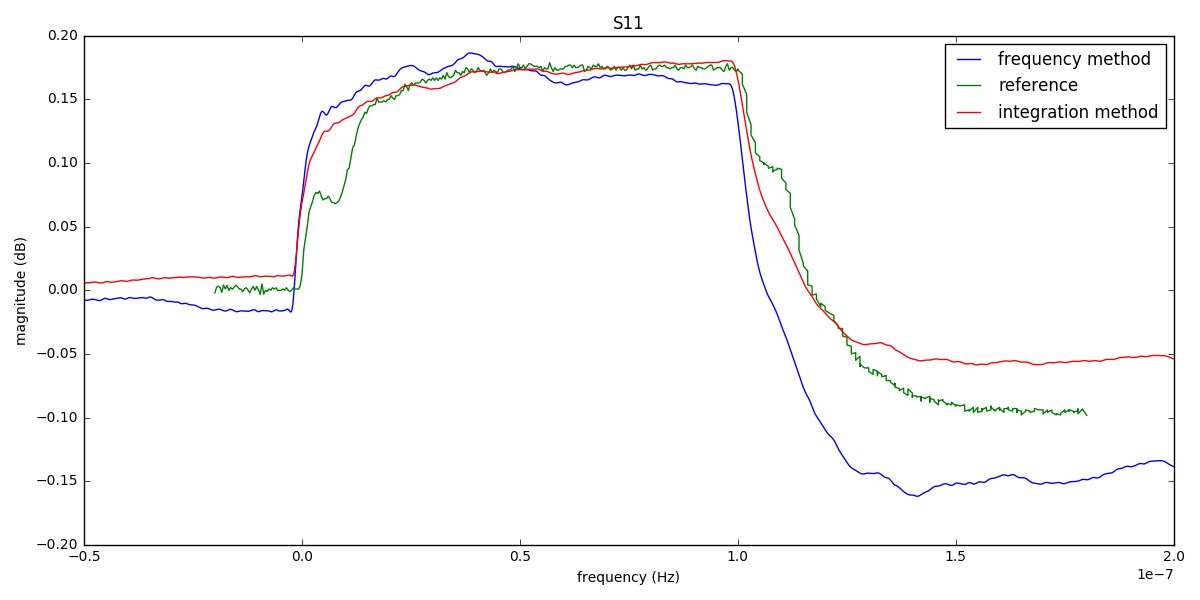
\includegraphics[width=0.9\textwidth]{src/3/figures/final_comparison_reconstructions.png}
  \caption{Reference current waveform versus frequency-domain and time-domain reconstructions}
  \label{fig:freq-domain-reconstructed}
\end{figure}
